\section{Скачивание, установка, запуск и настройка IDE Code::Blocks}

\subsection{Скачивание с http://www.codeblocks.org/downloads}

\begin{frame}[t]{Code::Blocks --- С/C++ IDE}


\includegraphics[width=0.2\textwidth]{logo}

\url{http://www.codeblocks.org} --- сайт Code::Blocks

\url{http://www.codeblocks.org/downloads/26} скачать:

  \begin{itemize}
    \item \textbf{codeblocks-13.12-setup.exe} - только среда разработки без компилятора и отладчика. 
    \item \textbf{codeblocks-13.12mingw-setup.exe} - IDE + MinGW (компилятор + отладчик).
    \item \textbf{codeblocks-13.12mingw-setup-TDM-GCC-481.exe} - IDE + Альтернативный компилятор и отладчик (TDM).
  \end{itemize}

  Выбирайте: \textbf{codeblocks-13.12mingw-setup.exe}

\end{frame}

\subsection{Установка Code::Blocks}

\begin{frame}[t]{Next > Next > Next}
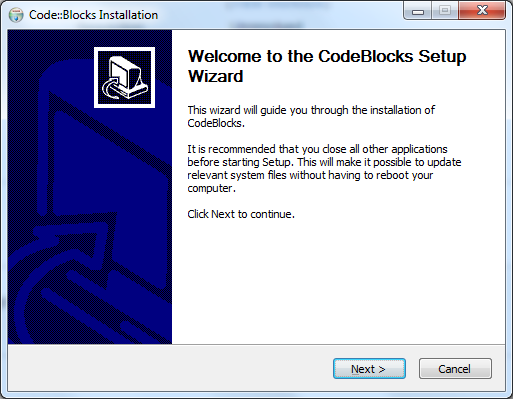
\includegraphics[width=0.5\textwidth]{00_codeblocks/step1.png}
\end{frame}

\begin{frame}[t]{GNU General Public License}
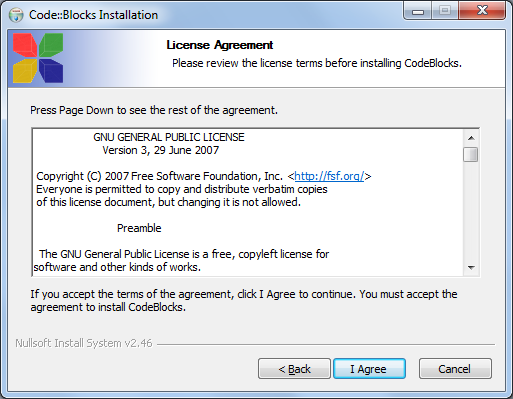
\includegraphics[width=0.5\textwidth]{00_codeblocks/step2.png}
\end{frame}

\subsection{Запуск Code::Blocks}

\begin{frame}[t]{Начальный экран Code::Blocks}
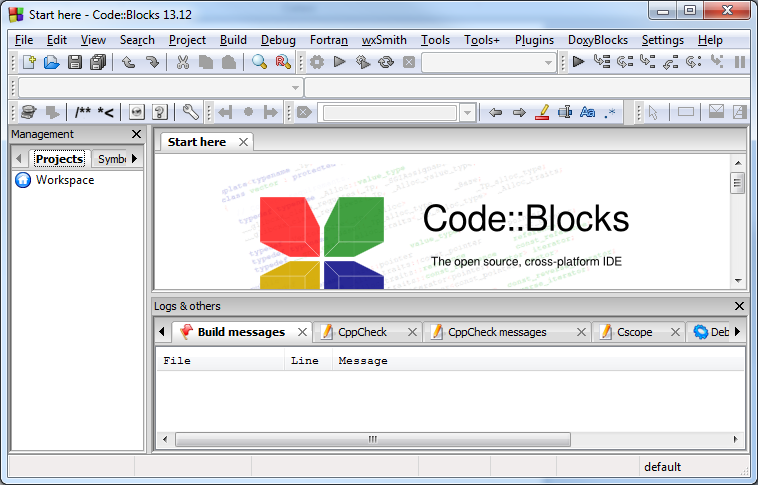
\includegraphics[width=0.7\textwidth]{00_codeblocks/CodeBlocks.png}
\end{frame}

\subsection{Настройка Code::Blocks}

\begin{frame}[t]{Настройки компиляторов для Code::Blocks}
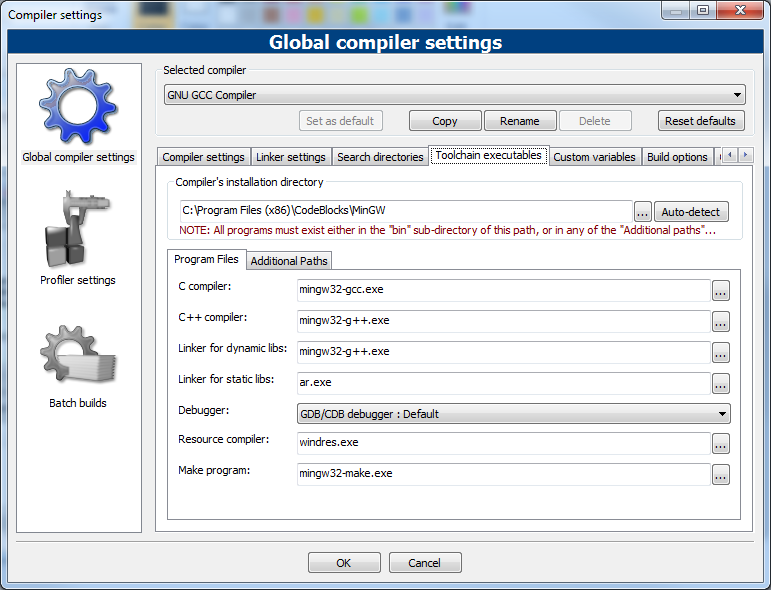
\includegraphics[width=\textwidth]{00_codeblocks/CodeBlocks_GlobalCompilerSettings.png}
\end{frame}

\subsection{Создание проекта в Code::Blocks}

\begin{frame}[t]{Начальный экран Code::Blocks}
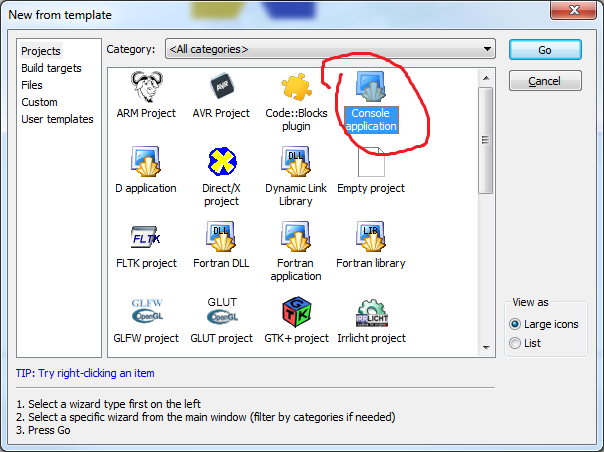
\includegraphics[width=\textwidth]{00_codeblocks/CodeBlocks_Console_application.png}
\end{frame}

\begin{frame}[t]{Выбираем язык программирования C или C++}
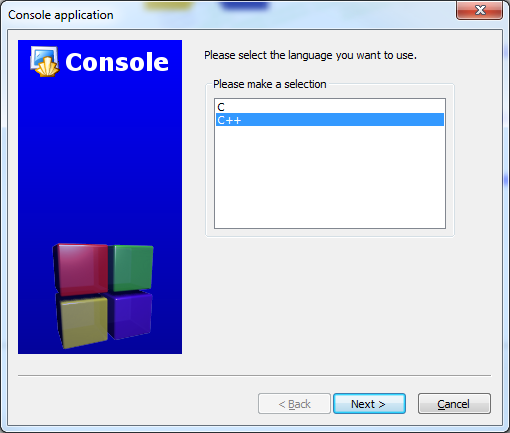
\includegraphics[width=\textwidth]{00_codeblocks/CodeBlocks_cpp.png}
\end{frame}

\subsection{Горячие клавиши / Hot Keys / Shortcuts}

\begin{frame}[t]{Горячие клавиши / Hot Keys / Shortcuts}
  Редактор:
  \begin{itemize}
    \item \textbf{Ctrl + Z} --- Отменить последнее действие. 
    \item \textbf{Ctrl + Shift + Z} --- Redo last action. 
    \item \textbf{Ctrl + X} --- Вырезать выделенный текст. 
    \item \textbf{Ctrl + C} --- Скопировать текст. 
    \item \textbf{Ctrl + V} --- Вставить текст. 
    \item \textbf{Ctrl + A} --- Выделить весь текст. 
    \item \textbf{F11} --- Переключение header / source. 
    \item \textbf{Ctrl + Shift + C} --- Закомментировать выделенный код. 
    \item \textbf{Ctrl + Shift + X} --- Раскомментировать выделенный код. 
    \item \textbf{Ctrl + Пробел} --- Автодополнение. 
    \item \textbf{Ctrl + B} --- Поставить закладку. 
    \item \textbf{Alt + PgUp} / \textbf{Alt + PgDown} --- Ходить по закладкам. 
  \end{itemize}
\end{frame}

\begin{frame}[t]{Горячие клавиши / Hot Keys / Shortcuts}
  Работа с файлами:
  \begin{itemize}
    \item \textbf{Ctrl + N} --- Новый файл или проект. 
    \item \textbf{Ctrl + O} --- Открыть файл или проект. 
    \item \textbf{Ctrl + S} --- Сохранить текущий файл. 
    \item \textbf{Ctrl + Shift + S} --- Сохранить все открытые файлы. 
    \item \textbf{Ctrl + F4} / \textbf{Ctrl + W} --- Закрыть текущий файл. 
    \item \textbf{Ctrl + Shift + F4} / \textbf{Ctrl + W} --- Закрыть текущий файл.     
  \end{itemize}
\end{frame}

\begin{frame}[t]{Сборка, запуск и отладка}
  Сборка и запуск:
  \begin{itemize}
    \item \textbf{Ctrl + F9} --- Компиляция. 
    \item \textbf{Ctrl + F10} --- Запуск программы. 
    \item \textbf{F9} --- Собрать и запустить. 
  \end{itemize}

  Отладка (Debug):
  \begin{itemize}
    \item \textbf{F8} --- Отладка. 
    \item \textbf{Ctrl + F7} --- Продолжить отладку. 
    \item \textbf{F7} --- Выполнить одну строку. 
    \item \textbf{Shift + F7} --- Выполнить строку с входом внутрь. 
    \item \textbf{Ctrl + Shift + F7} --- Выполнить до конца функции. 
    \item \textbf{F5} --- Включить/выключить точку останова (breakpoint). 
    \item \textbf{F4} --- Выполнить до курсора. 
  \end{itemize}
\end{frame}